\documentclass[11pt]{article}
\usepackage{titlesec}
\usepackage{graphicx}
\usepackage{float}
\usepackage{sectsty}
\usepackage[a4paper, total={6in, 9in}]{geometry}
\usepackage[hidelinks]{hyperref}
\usepackage{longtable}
% \subsectionfont{\normalfont\large\itshape\underline}
% \paragraphfont{\normalfont\itshape}
\setlength{\parskip}{1em}



\graphicspath{ {images/} }

\author{Nathan}
\date{\today}
\title{Prototype designs for cost effective continuous weighing systems}

\setcounter{secnumdepth}{4}
\titleformat{\paragraph}
{\normalfont\normalsize\bfseries}{\theparagraph}{1em}{}
\titlespacing*{\paragraph}
{0pt}{3.25ex plus 1ex minus .2ex}{1.5ex plus .2ex}

\begin{document}

\maketitle
\clearpage 
\tableofcontents
\clearpage

%%%%%%%%%%%%%%%%%%%%%%% Intro%%%%%%%%%%%%%%%%%%%%%%%%%%%%%%%%
\section{Introduction}
Compartment 7 in our smart-house aims to be a sophisticated gravimetrics system, where plants can be under controlled
environments, automatically weighed and watered over time.

\par

Typically this would require very precise, expensive and specialist equipment to perform. Our aim is to find a
cost effective way to do this. We will be working off the rough idea that a professional implementation would cost in the
range of \pounds1000 per plant, at current we have space for and aim to facilitate up-to 120 plants at any-one time therefore a
complete system with a cost lower than \textsterling1000 per plant and/or an overall cost less than \textsterling120,000

\par

At current we have the facility to read the weight of each individual plant, water and collect information into a
database. However some issues have been uncovered that make this system unsuitable for scientific experiments.
\subsection{What is the problem with the current solution?}
The main issue that we have encountered when working with the current implementation is that some
of the weighing results that we gathered were seeming off and inconsistent with previous readings
and expectations. Investigation into this led us to believe that the typical load-cell used in a
laboratory scale are ill-suited for continuous weighing.

\par

Load-cells by their nature are very sensitive to changes in their environment in particular temperature.
In a green-house environment this quickly becomes a problem. Through a series of tests we discovered a
potential drift in scale readings of \(\pm10\%\)

\subsection{Why a software approach isn't possible}
TODO
\subsection{How a hardware approach could be the solution}
TODO

%%%%%%%%%%%%%%%%%%%%%%% Solutions%%%%%%%%%%%%%%%%%%%%%%%%%%%%%%
\section{Solutions}
For each of these proposed solutions we work off some assumptions about the weights that we will be working with.
At most we can assume we will not have to handle plants that are over 10kg in weight, and we would take into account that
each scale is around 1kg as well. At current our benches/tables consist of 2$\times$2 smaller benches.
Each of these smaller benches hold 4 plants so we will aim for each section of a bench to hold/lift a minimum of 44kg and for a complete bench to hold/lift a minimum of 176kg. To be safe our prototypes will aim above this where possible within the scope.

\subsection{Linear Actuators}
The use of linear actuators would use electrically powered stepper motors to produce upwards or
downwards movements. 
\subsubsection{Design}
When using linear actuators we have two options, either lift the plants from the balances, or else lift the balances to the
plants. I think both are viable options and that by prototyping both options we can better see which has a more practical
application within the Gravimetrics system. 

\paragraph{Lifting balances}\mbox{}\\
Here we would lift a load-cell (the cylinder) up to a plat above it. This method allows for the loadcells
to be given some time without being stressed with weights on them (which could damage the hardware if left in constant strain). 

\begin{figure}[H]
  \begin{center}
    \includegraphics[width=150px]{linear2}
    \caption{Lifting scales to the plants using actuators}
  \end{center}
\end{figure}

\paragraph{Lifting plants}\mbox{}\\
Alternately we could attempt to lift the plants themselves. This could be more simple to implement.
Holding the plants above the load cells using the actuators would not necessarily be a strain as
they are perfectly capable of holding at a specific height.

\begin{figure}[H]
  \begin{center}
    \includegraphics[width=150px]{linear}
    \caption{Lifting plants using actuators}
  \end{center}
\end{figure}

\subsubsection{Prototype Proposal}
For the prototype of this system we would hope to be able to lift a single bench of 4 plants a minimum of 10mm away from
the load-cells. Too small a movement and we run the risk of a dip in the bench material due to weight. We must also take into account
the possibility of losing track of the current actuator height and so under/over lifting needs to have buffer room which anything less than 10mm
couldn't provide comfortably. 
\paragraph{Parts List}

\begin{center}
  \begin{longtable}{||c |  p{0.25\linewidth}   |c | c | c||} 
    \hline
    Part & Supplier & Part No & Quantity & Price \\ [0.5ex] 
    \hline\hline
    Linear Actuator & RS & 764-3471 & 1 & \pounds176.69 \\ 
    \hline
    Actuator Controller & RS & 918-1372 & 1  & \pounds48.64 \\
    \hline
    Various fittings & RS & X & X &  \pounds15 \\
    \hline
    \hline
    Total & & & & \pounds240.33 \\
    \hline
  \end{longtable}
\end{center}

\paragraph{Estimated Cost} \mbox{}\\
TODO
\subsubsection{Benefits}
TODO
\subsubsection{Possible issues}
TODO
\paragraph{Maintainability}\mbox{}\\
TODO

\subsection{Scissor Jack}
The scissor jack is perhaps one of the simplest mechanisms and would require the least amount of work in order to setup a
brief example. However it would require the user to manually move it initially (However a DC motor could be used in the
future to provide and more automated mechanism). 
\subsubsection{Design}
The design again being simple would require the load-cell to be balanced upon the scissor jack, we then apply a turning
motion to raise the balance to the plants which by taking the weight of the plant pot (cut through the table) we can proceed
to read the weight of the load cells. 

\begin{figure}[H]
  \begin{center}
    \includegraphics[width=150px]{bench2}
    \caption{Lifting scales to the plants using actuators}
  \end{center}
\end{figure}


\subsubsection{Prototype Proposal}
For this proposed prototype all we require (that is unique to this prototype) is the scissor jack itself. Other materials
such as aluminium for the frame of the holder and lifter is something that we can re-use between prototypes. 
\paragraph{Parts List}\mbox{}\\

\begin{center}
  \begin{longtable}{||c |  p{0.25\linewidth}   |c | c | c||} 
    \hline
    Part & Supplier & Part No & Quantity & Price \\ [0.5ex] 
    \hline\hline
    Scissor Jack & Screwfix & 97595 & 2 & \pounds14.99 \\ 
    \hline
    \hline
    Total & & & & \pounds29.98 \\
    \hline
  \end{longtable}
\end{center}

\paragraph{Estimated Cost}\mbox{}\\
The main cost of this is the scissor jack, in addition to smaller parts that are not important to mention I would suggest
that the price of this setup to be <\pounds30, with the majority being between some aluminium frames and the scissor jack itself. 
\subsubsection{Benefits}

The main benefits of using this type of system are:
\begin{itemize}
  \item Cheap to setup
  \item Room to expand to become automated
  \item Easily maintained
  \item Parts are widely available and manufacturer doesn't matter 
\end{itemize}

\subsubsection{Possible issues}

The foreseeable issues are:  
\begin{itemize}
  \item Not initially automated
  \item Accurately and consistently turning a motor a specific am mount can be  
  
\end{itemize}


\paragraph{Maintainability}
TODO

\subsection{Hanging Basket}
TODO
\subsubsection{Design}

\begin{figure}[H]
  \begin{center}
    \includegraphics[width=150px]{basket}
    \caption{Holding the plants in a basket, with an S-Beam load-cell}
  \end{center}
\end{figure}

\subsubsection{Prototype Proposal}
TODO
\paragraph{Parts List}\mbox{}\\

\begin{center}
  \begin{longtable}{||c |  p{0.25\linewidth}   |c | c | c||} 
    \hline
    Part & Supplier & Part No & Quantity & Price \\ [0.5ex] 
    \hline\hline
    Hanging-basket & Homebase & 428809 & 1 & \pounds1.99 \\
    \hline
    S-Beam load-cell & Omega & LCM101 & 1 & \pounds222.00 \\
    \hline
    Amplifier Board & Omega & TXDIN1600S & 1 & \pounds133 \\
    \hline
    \hline
    Total & & & & \pounds356.99 \\
    \hline
  \end{longtable}
\end{center}
\paragraph{Estimated Cost}\mbox{}\\
TODO
\subsubsection{Benefits}
TODO
\subsubsection{Possible issues}
TODO
\paragraph{Maintainability}\mbox{}\\
TODO

\subsection{Alternate Load-Cell}
TODO
\subsubsection{Design}
TODO
\subsubsection{Prototype Proposal}
TODO
\paragraph{Parts List}\mbox{}\\

\begin{center}
    \begin{longtable}{||c | p{0.25\linewidth}   |p{0.25\linewidth} | c | c||} 
      \hline
      Part & Supplier & Part No & Quantity & Price \\ [0.5ex] 
      \hline\hline
      Load-cell & Omega & LCM501  & 1 & \pounds249 \\ 
      \hline
      Amplifier Board & Omega & TXDIN1600S & 1 & N/A \\
      \hline
      \hline
      Total & & & & \pounds249 \\
      \hline
    \end{longtable}
\end{center}

Both prototype load-cell designs can share an amplifier board as the expense is too much to have duplicate components.

\paragraph{Estimated Cost}\mbox{}\\
TODO
\subsubsection{Benefits}
TODO
\subsubsection{Possible issues}
TODO
\paragraph{Maintainability}\mbox{}\\

\subsection{Pneumatic lifting}
Pneumatics could be potential solution in that the majority of the cost is in the initial setup.
Once a suitable air compressor is available, connecting additional valves and cylinders is very economical. 
\subsubsection{Design}
For the design I would be using a setup that is rather simple and borrow a lot from the linear actuators, the main difference
being that this design would incorporate air compressors and pumps in place of electrical powered actuators.

\par

In the diagram given, we can see an air compressor controlled by a servo controller providing a connection to the actuator, these would be controlled by a micro-controller device.

\begin{figure}[H]
  \begin{center}
    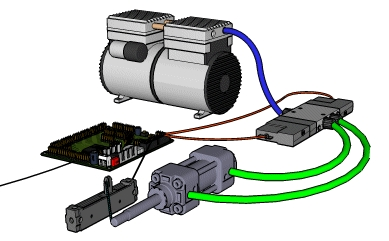
\includegraphics{pneSetup}
    
    \caption{Basic Pneumatic setup using air compressor, servo controller and
      cylinder\cite{dnicky}}
  \end{center}
\end{figure}

\subsubsection{Prototype Proposal}
\paragraph{Parts List}\mbox{}\\

\begin{center}
    \begin{longtable}{||c | p{0.25\linewidth}   |p{0.25\linewidth} | c | c||} 
      \hline
      Part & Supplier & Part No & Quantity & Price \\ [0.5ex] 
      \hline\hline
      Short-stroke cylinder & Festo & ADVC-32-10-I-P-A  & 1 & N/A \\ 
      \hline
      Joining Connectors & RS & 812-156 & 4 & \pounds2.40 \\
      \hline
      Extruded Aluminium & aluminium-profile &  466-7219 & 4 & \pounds17.99\\
      \hline
      Solenoid & RS &  839-3161 & 1 & \pounds78.26\\
      \hline
      Solenoid Connector & RS & 484-010 & 1 & \pounds1.87 \\ [1ex] 
      \hline
      \hline
      Total & & & & \pounds161.69\\
      \hline
    \end{longtable}
\end{center}

\paragraph{Estimated Cost}\mbox{}\\
The estimated costs for this prototype would be around \pounds100.52 although additional cost is not calculated for the creating of an additional hook-up point for the current pump.
\subsubsection{Benefits}
\subsubsection{Possible issues}
\paragraph{Maintainability}\mbox{}\\


%%%%%%%%%General parts required for all prototypes %%%%%%%%%%%%
\subsection{General Parts required} 
\begin{center}
    \begin{longtable}{||c | p{0.25\linewidth}   |p{0.25\linewidth} | c | c||} 
      \hline
      Part & Supplier & Part No & Quantity & Price \\ [0.5ex] 
      \hline\hline
      Extruded Aluminium & aluminium-profile &  466-7219 & 4 & \pounds17.99\\
      \hline
      Stripboard & RS & 100-4328 & 3 & \pounds3.41\\
      \hline
      \hline
      Total & & & & \pounds82.19\\
      \hline
    \end{longtable}
\end{center}



%%%%%%%%%%%%%%%%%%%%%%% Conclusion%%%%%%%%%%%%%%%%%%%%%%%%%%%%
\section{Conclusion}

\subsection{Total Costs for Prototypes}

\begin{center}

  \begin{longtable}{||c|c||}
    \hline
    Prototype & Cost \\ [0.5ex]
    \hline \hline
    Linear Actuators & \pounds240.33\\
    \hline
    Scissor Jack & \pounds29.98\\
    \hline
    Hanging Basket & \pounds356.99 \\
    \hline
    Alternate load-cell &\pounds249 \\
    \hline
    Pneumatics lifting & \pounds161.69 \\ 
    \hline
    General parts & \pounds 82.19
    \hline
    Total & \pounds1120.18 \\
    \hline
  \end{longtable}

\end{center} 

\subsection{Best suited solution}


%%%%%%%%%%%%%%%%%%%%%%% References%%%%%%%%%%%%%%%%%%%%%%%%%%%%
\begin{thebibliography}{9}
  
\bibitem{dnicky} 
  User of indestructibles website, user dnicky,
  \url{http://www.instructables.com/id/Arduino-Pneumatic-Flight-Simulator}
\end{thebibliography}

\end{document}